%Desarrollo e implementación
\section{Programación y documentación}
Este apartado tiene como objetivo describir en qué consiste el desarrollo y documentación asociado a una parte del sistema a mostrar, para ejemplificar a partir de las historias de usuario involucradas, cómo es la forma de trabajo.
	

Se ha seleccionado dos \textit{EPICS} del sistema, que a continuación se detalla, para describirlos, el código desarrollado se encuentra en el \textbf{Anexo \ref{codigo}}
\begin{enumerate}
\item \textit{\textbf{Permitir al usuario añadir los análisis realizados }}
%(Perfil de mediciones con carga sencilla de mediciones Carga de mediciones completa incluyendo a los analisis.

\textbf{User Stories relacionados}
    \begin{itemize}
        \item \textbf{US-2 }Como paciente, quiero añadir al sistema los estudios realizados para evitar posibles perdidas.
        \item \textbf{US-5 }Como paciente quiero que los sistemas de salud existentes puedan cargar sus resultados directamente en mi carpeta de salud para centralizar mi información
        \item  \textbf{US-7} Como paciente quiero categorizar mis estudios por rama de medicina, para lograr una mejor organización y navegabilidad en el sistema
        \item \textbf{US-8} Como laboratorio, quiero cargar información de un paciente en su cuenta para ahorrarle las molestias de volver
    \end{itemize}
\item \textbf{\textit{Permitir a los usuarios generar vistas de su información a lo largo del tiempo, a través de gráficas , tablas y resúmenes }}
%(Histórico de mediciones que permite ver el avance de las mediciones).

\textbf{User Stories relacionados}
    \begin{itemize}
        \item \textbf{US-17} Como paciente quiero ver gráficas que resuman mi información en particular para poder ver mis cambios a lo largo de la historia.
        \item \textbf{US-15} Como médico quiero ver gráficas que resuman la información de un paciente para poder ver sus cambios a lo largo de la historia y así apoyar la toma de decisiones y el diagnóstico.
    \end{itemize}
\end{enumerate}

{\scriptsize
	\begin{center} %sidewaystable
		\centering
		%\begin{adjustbox}{max width=\textheight}
		\resizebox{\textwidth}{!}{
			\begin{tabular}{|l|l|}
				\hline 
				\rowcolor[gray]{0.9} 
				\multicolumn{2}{|c|}{\textbf{Plantilla de programación}} \\
				\hline
				\textbf{Denominación del programa} &
				YesDoc \\
				\hline       
				\textbf{User Sories} &
				US-2, US-5, US-7, US-8, US-15, US-17\\
				\hline
				\textbf{Fecha de inicio de la programación} & 11 de septiembre del 2015\\
				\hline
				\textbf{Fecha de finalización} & 17 de octubre del 2015\\
				\hline
				\textbf{Tiempo dedicado} & 65hs\\
				\hline
				\textbf{Nombre y Apellido de programadores} & Michael Manganiello, Ivan Terreno\\
				\hline
				\textbf{Usuarios que aprobaron} & Yanina Morales, Franco Canizo\\
				\hline
				
			\end{tabular}
		}	%\end{adjustbox}
	\end{center}
}

\begin{comment}
denominación del programa, caso de uso del que proviene, fecha de inicio de la programación, fecha de finalización, casos de prueba utilizados, clases involucradas, nombre y apellido del programador, del usuario que aprobó
\end{comment}

\subsection{Descripción de la funcionalidad} % ya se dijo en el sprint
\subsubsection{Cargar análisis}

 La definición de un análisis permite al usuario reunir una serie de mediciones y darles un motivo que destaque la razón por la cual se tomó dicha medida. Así un usuario podría indicar el análisis que reúne las medidas diarias de presión o las medidas de presión, peso y azúcar que forman parte de los controles diarios que se realiza un usuario. Por otro lado un médico puede ingresar el conjunto de medidas que formaron parte del proceso de diagnóstico de una persona o el mismo paciente, una vez terminada la consulta podría crear un análisis indicando el motivo y reuniendo los resultados de mediciones tomadas manualmente.

\subsubsection{Generación de tablas y gráficas de mediciones}

Para una vista rápida e intuitiva de las medidas se trabaja para generar gráficas y tablas que resumen los datos de medidas tomadas manualmente y cargadas a la aplicación.

\subsection{Diseño Técnico}
En este documento se efectúa un diseño lógico que permite, a partir de la arquitectura y la descripción del requisito en la fase de análisis, dar soporte a la implementación de la funcionalidad.

Aquí se describen los artificios utilizados a nivel técnico para resolver el problema que se planteó en la historia de usuario. Se incluyen diagrmas de clases, modelos de datos, etc. Para esto se utiliza un documento compuesto de 4 partes
\begin{itemize}
\item Objetivo

El objetivo consiste en poder cargar mediciones de distintos tipos, de diferentes fuente y en diferentes unidades a los análisis que vaya generando el usuario y van quedando relacionados al perfil creado al registrarse.

\item Diseño de a fase de datos

Se requiere la preparación de datos para popular las tablas que guardan los datos de los objetos de las siguientes clases, \textbf{[Figura \ref{clases-doc-prog}]}.

    \begin{figure}[h]
        \centering
        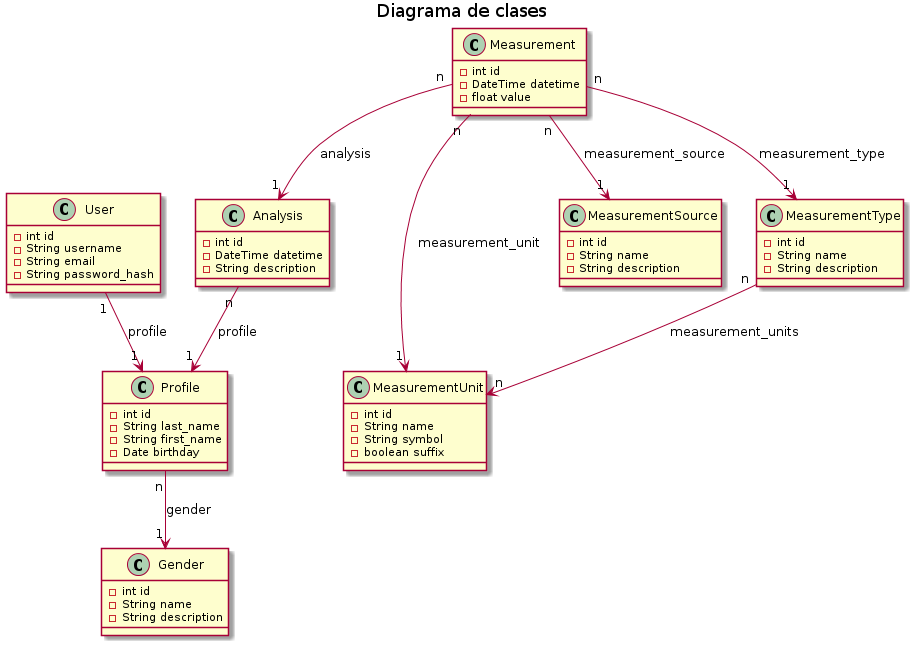
\includegraphics[width=0.5\textwidth]{img/dc_mediciones}
        \caption{DC-Mediciones}
		\label{clases-doc-prog}
    \end{figure}

\newpage

\item Diseño API REST

%------------------------ API REST --------------------------------

La estructura de nuestra api busca aplicar lo más fielmente posible el principio arquitectónico que define  REST, Representational State Transfer, el cual consiste en un estilo de arquitectura de software para construir web services escalables. La comunicación con la api es a través del protocolo HTTP y se busca utilizar los mismos verbos, GET, POST, PUT, entre otros. Para que la API sea REST cumple con las siguientes 6 restricciones según establece el paper que introduce REST:
\begin{enumerate}
	\item Cliente-Servidor
    
    La API debe estar separada del cliente y se comunican a través del protocolo de red HTTP.
    
    \item Stateless
    
    No se mantienen sesiones, cada solicitud y respuesta están totalmente aisladas unas de otras. Los clientes deben ser autenticados en cada solicitud. Un gris en stateless podría ser usar cookies para almacenar información que se mantiene entre solicitudes.
    
    \item Cache
    
    El servidor debe proveer directivas de cacheo que indiquen a intermediarios las condiciones bajo las cuales cachear información.
    
    \item Uniform interface
    
    \textbf{Identificación de recursos}, los recursos son todas las entidades en el dominio de nuestra aplicación. Cada recurso tiene un único identificador (URL), accediendo a los identificadores podemos obtener colecciones de representación de recursos.
    
    \textbf{Representación de recursos}, el cliente se comunica y opera con los recursos a través de las representaciones que la api ofrece. Las representaciones pueden presentarse en distintos formatos (en nuestro caso JSON). Las representaciones se separan de los recursos.
    
    \textbf{Mensajes descriptivos}, tanto solicitudes como respuestas cliente-servidor están aisladas completamente por lo que no hay información relacionada entre sucesivas solicitudes y respuestas.
    
    \textbf{Hypermedia}, plantea una forma de usar la api a través de enlaces, el cliente descubre nuevos recursos a través de la información que brindan los recursos previamente descubiertos.
    
    \item Layered system
    Cliente y servidor no necesariamente se comunican directamente, pueden existir intermediarios.
    
    \item Code on demand
    Restricción opcional, el servidor provee código que el cliente puede utilizar.
    
\end{enumerate}
\end{itemize}
La estructura de nuestra API se presenta de la siguiente forma:

\begin{comment}
		imagen directorios	contenidos...
\end{comment}



Uno de los archivos principales es el archivo de configuración, Flask no necesita mucha configuración, solo una serie de pares clave-valor. En nuestra aplicación tenemos 4 modos en los que puede correr la aplicación. development, staging, testing and production.

Lo que hacemos es definir una clase principal Config donde colocamos las variables de configuración que aplicarán a todas las configuraciones, y luego tres subclases enlas cuales determinamos configuraciones que son específicas para cada uno de los tipos de configuración. La clave Secret key la usamos para encriptación de todas las fuentes. Tanto flask como las extensiones usan secret key para encriptar.

Para definir el modo de configuración el valor lo tomamos de una variable del environment y como mostramos en el código, la configuración por defecto es la de producción.
    
\begin{lstlisting}[language=Python]
class Config(object):
    DEBUG = False
    TESTING = False
    CSRF_ENABLED = True
    # encriptacion de todas las fuentes
    SECRET_KEY = 'this-really-needs-to-be-changed'
    SQLALCHEMY_DATABASE_URI = os.environ.get('DATABASE_URL', 'postgresql:///salud_dev?client_encoding=utf8')
    Parametro que indica si el parser de argumentos debe devolver la totalidad de los errores encontrados en una
    peticion a la API (True), o solo el primer error (False).
    BUNDLE_ERRORS = True
    # Directorio donde guardaremos el archivo
    #UPLOAD_FOLDER = '/tmp'
    #ALLOWED_IMG_EXTENSIONS = set(['png'])
    UPLOADED_PHOTOS_DEST = '/tmp/imagenes'
    MAX_CONT_IMG_LENGTH = 6 * 1024 * 1024
    uploaded_photos = UploadSet('photos', IMAGES)
    # Claves, publica y privada, de autenticacion de la aplicacion en Dropbox.
    DROPBOX_APP_KEY = 'i7u47ht1t730nar'
    DROPBOX_APP_SECRET = os.environ.get('DROPBOX_APP_SECRET', '')

class ProductionConfig(Config):
    DEBUG = False

class StagingConfig(Config):
    DEVELOPMENT = True
    DEBUG = True
    
class DevelopmentConfig(Config):
    DEVELOPMENT = True
    DEBUG = True
    
class TestingConfig(Config):
    TESTING = True
\end{lstlisting}

Otro de los archivos importantes es el que presenta el código de inicio de la aplicación, en este encontramos tres puntos principales, en primer lugar la creación de la instancia de flask para nuestra api

\begin{lstlisting}[language=Python]
app = Flask(__name__)
flask_config_mode = os.getenv('FLASK_CONFIG_MODE', 'production')
app.config.from_object(get_config_class(flask_config_mode))
\end{lstlisting}

El punto donde definimos los identificadores para acceder a un determinado recurso, usando el método add\_resource de la extensión de flask, \textbf{flaskRESTful} que nos permite registrar una ruta en flask. Esto permite que nuestra API presente una interfaz única.

\begin{lstlisting}
api.add_resource(GenderView, '/genders/<int:id>')
api.add_resource(GenderList, '/genders')
api.add_resource(ProfileView, '/profiles/<int:id>')
api.add_resource(ProfileList, '/profiles')
api.add_resource(MeasurementView, '/measurements/<int:id>')
api.add_resource(MeasurementList, '/measurements')
api.add_resource(MeasurementSourceView, '/measurement_sources/<int:id>')
api.add_resource(MeasurementSourceList, '/measurement_sources')
api.add_resource(MeasurementTypeView, '/measurement_types/<int:id>')
api.add_resource(MeasurementTypeList, '/measurement_types')
api.add_resource(MeasurementUnitView, '/measurement_units/<int:id>')
api.add_resource(MeasurementUnitList, '/measurement_units')
api.add_resource(PermissionTypeList, '/permission_types')
\end{lstlisting}

\begin{sloppypar}
Cabe destacar que las rutas expuestas presentan un resumen y no la totalidad de rutas que presenta actualmente la API.
Como podemos observar, el cliente tendrá acceso a la representación de respuesta del recurso MeasurementList solo enviando una representación correcta en una solicitud a la URL \url{http://dominio_raiz/measurements}.
\end{sloppypar}

Por último, el tercer punto, se ubica en otro archivo y nos permite iniciar la API.

\begin{lstlisting}[language=Python]
#!flask/bin/python

# -*- coding: utf-8 -*-

from app import app

if __name__ == '__main__':
    app.run(host='0.0.0.0')
\end{lstlisting}

Ejecutando este script de python iniciamos la API.
Los recursos de la API presentan la siguiente estructura:

\begin{lstlisting}[language=Python]
class MeasurementList(Resource):
    @marshal_with(MeasurementFields.resource_fields, envelope='resource')
    def get(self):
        measurements = Measurement.query.all()
        return measurements
    @marshal_with(MeasurementFields.resource_fields, envelope='resource')
    def post(self):
        args = parser_post.parse_args()
        new_measurement = Measurement(args['datetime'],
                                      args['value'],
                                      args['analysis_id'],
                                      args['profile_id'],
                                      args['measurement_source_id'],
                                      args['measurement_type_id'],
                                      args['measurement_unit_id'])
        db.session.add(new_measurement)
        db.session.commit()
        return new_measurement, 201
\end{lstlisting}

Como vemos el recurso define dos métodos, uno con el nombre \texttt{get} y otro con el nombre \texttt{post}.
Estos métodos responden a las solicitudes HTTP al identificador \texttt{/measurements}, que indiquen en el atributo method el operador GET y POST respectivamente. En el caso del recurso indicado, la solicitud con operando GET devolverá al cliente una colección de representaciones de medidas en la base de datos mientras que con el operando POST cargará una nueva medida.

La clase del modelo que para las medidas se encuentra en el paquete models del paquete mod\_profiles

\begin{lstlisting}[language=Python]
class Measurement(db.Model):
    # Attributos, columnas de la base de datos
    id       = db.Column(db.Integer, primary_key=True)
    datetime = db.Column(db.DateTime)
    value    = db.Column(db.Float)
    # Claves foraneas
    analysis_id           = db.Column(db.Integer, db.ForeignKey('analysis.id'))
    profile_id            = db.Column(db.Integer, db.ForeignKey('profile.id'))
    measurement_source_id = db.Column(db.Integer, db.ForeignKey('measurement_source.id'))
    measurement_type_id   = db.Column(db.Integer, db.ForeignKey('measurement_type.id'))
    measurement_unit_id   = db.Column(db.Integer, db.ForeignKey('measurement_unit.id'))
    # Relaciones entre tablas
    analysis           = db.relationship('Analysis',
                                         backref=db.backref('measurements', lazy='dynamic'))
    profile            = db.relationship('Profile',
                                         backref=db.backref('measurements', lazy='dynamic'))
    measurement_source = db.relationship('MeasurementSource',
                                         backref=db.backref('measurements', lazy='dynamic'))
    measurement_type   = db.relationship('MeasurementType',
                                         backref=db.backref('measurements', lazy='dynamic'))
    measurement_unit   = db.relationship('MeasurementUnit',
                                         backref=db.backref('measurements', lazy='dynamic'))
    # Constructor de la clase
    def __init__(self, datetime, value, analysis_id, profile_id, source_id, type_id, unit_id):
        self.datetime              = datetime
        self.value                 = value
        self.analysis_id           = analysis_id
        self.profile_id            = profile_id
        self.measurement_source_id = source_id
        self.measurement_type_id   = type_id
        self.measurement_unit_id   = unit_id
    # Representacion string de la instancia
    def __repr__(self):
        return '<Measurement: %r>' % (self.datetime)
\end{lstlisting}

La definición de la clase del modelo se hace de acuerdo a lo que establece el ORM usado por el equipo, \textbf{SQLAlchemy}.

El nombre de la tabla en la base de datos se genera automáticamente cambiando CamelCase por camel\_case, el atributo column define la columna de la base de datos y las restricciones que se aplican a la misma, el atributo relationship define la relación entre las distintas tablas.

Como establecimos en la introducción de REST, la API funciona recibiendo solicitudes HTTP y respondiendo a las mismas. La API define identificadores a los cuales los clientes pueden referir, para que las solicitudes sean aceptadas. Éstas deben enviar información en el cuerpo que esté de acuerdo a las representaciones que definimos para la API, en nuestro caso, las representaciones deben ser del tipo JSON y tener los pares clave-valor que define el parser del recurso en el paquete parsers en common. Para el caso actual de medidas se define el siguiente parser.

\begin{lstlisting}[language=Python]
# Parser general
parser = reqparse.RequestParser()
parser.add_argument('datetime', type=is_valid_previous_datetime, required=True)
parser.add_argument('value', type=float, required=True)
parser.add_argument('analysis_id', type=is_valid_id, required=True)
parser.add_argument('profile_id', type=is_valid_id, required=True)
parser.add_argument('measurement_source_id', type=is_valid_id)
parser.add_argument('measurement_type_id', type=is_valid_id, required=True)
parser.add_argument('measurement_unit_id', type=is_valid_id, required=True)

# Parser para recurso POST
parser_post = parser.copy()

# Parser para recurso PUT
parser_put = parser.copy()

# Parser para recurso POST con usuario autenticado
parser_post_auth = parser.copy().remove_argument('profile_id')
\end{lstlisting}

Como podemos ver en la tercer línea, la API recibe un dato con el nombre ‘datetime’, el cual es un dato de carácter obligatorio que en caso de que no esté lanzará una excepción y será validado  por el método ``is\_valid\_previous\_datetime''. Este parser es usado en el método POST para sanear los datos recibidos de la solicitud y poder armar el objeto cuyos datos serán luego almacenados en la base de datos. Para el parseo de datos usamos la interfaz \textbf{Request Parsing} de flask-RESTful el cual valida los datos entrantes en la solicitud y los deserializa en objetos a nivel de la API.

Así como manejamos las representaciones para recibir solicitudes también definimos representaciones para las respuestas de la API en el paquete fields del directorio common. La clase define como serializar los objetos a nivel de la app a objetos con datos de tipo primitivos que luego son formateados a JSON (Javascript object notation) para devolverse en el cuerpo de la respuesta HTTP.

\begin{lstlisting}[language=Python]
class MeasurementFields:
    # Definicion de campos de la representacion de respuesta
    resource_fields = {
        'id': fields.Integer,
        'datetime': fields.DateTime(dt_format='iso8601'),
        'value': fields.Float,
        'analysis': fields.Nested(AnalysisFields.resource_fields),
        'profile': fields.Nested(ProfileFields.resource_fields),
        'measurement_source': fields.Nested(MeasurementSourceFields.resource_fields),
        'measurement_type': fields.Nested(MeasurementTypeFields.resource_fields),
        'measurement_unit': fields.Nested(MeasurementUnitFields.resource_fields),
    }
    # Definicion de campos requeridos
    required = ['id',
                'datetime',
                'value',
                'analysis',
                'profile',
                'measurement_type',
                'measurement_unit']
\end{lstlisting}

Para la serialización de datos usamos el decorador \textbf{marshal\_with} que define flask-restful.

El proceso de serialización lo inicia el decorador @marshal\_with, toma los datos que pueden estar en formato de diccionario, lista, objeto, un diccionario con los campos a entregar y devuelve los datos envueltos en un JSON. Ademas de contener la representación en el cuerpo, la respuesta contiene un código que determina si la solicitud se procesó satisfactoriamente o no utilizando los códigos de error que define HTTP.

\begin{lstlisting}[language=Python]
class MeasurementList(Resource):
    @marshal_with(MeasurementFields.resource_fields, envelope='resource')
    def post(self):
        args = parser_post.parse_args()
        new_measurement = Measurement(args['datetime'],
                                      args['value'],
                                      args['analysis_id'],
                                      args['profile_id'],
                                      args['measurement_source_id'],
                                      args['measurement_type_id'],
                                      args['measurement_unit_id'])
        db.session.add(new_measurement)
        db.session.commit()
        return new_measurement, 201
\end{lstlisting}

 Como podemos ver en el código del método post del recurso para las medidas utilizamos parser para manejar las representaciones de solicitudes y marshal\_with para manejar las representaciones de respuesta. Esta definición de representaciones de solicitud y de respuesta hacen que nuestra API brinde una interfaz uniforme cumpliendo con la restricción establecida por la arquitectura REST. 
 Este desarrollo se repite para los recursos de las clases de nuestro modelo.

%---------------------------FIN API REST-------------------------

	contenidos...



\subsubsection{Objetivo}
El objetivo de este documento consiste en describir técnicamente el diseño de la solución planteada para poder implementar en la aplicación la carga y muestra de análisis.

\subsubsection{Descripcion}%acaaaaaaaa



\subsection{Técnicas de programación utilizadas}
\subsection{Entorno, herramientas y tecnologías utilizadas}
%LO HICIMOS EN OTRO LADO!!!!!!
\subsection{Código fuente}

Lo primero que definimos son los \textbf{modelos}, debemos tener en cuenta que la función que cumplen estos modelos fue descripta en cada sprint, los modelos de medidas en el \textbf{sprint-3}, usuarios y perfiles en el \textbf{sprint-5}, gestión de análisis \textbf{sprint-6}. Los modelos desarrollados son los siguientes.

\begin{enumerate}
\item \textbf{Gender}
	
\begin{lstlisting}[language=Python]
class Gender(db.Model):
    # Attributes
    id          = db.Column(db.Integer, primary_key=True)
    name        = db.Column(db.String(50), unique=True)
    description = db.Column(db.String(255))
	# Constructor
    def __init__(self, name, description):
        self.name        = name
        self.description = description
	# Class string representation
    def __repr__(self):
        return '<Gender: %r>' % (self.name)
\end{lstlisting}
	
\item \textbf{User}
	
\begin{lstlisting}[language=Python]
class User(db.Model):
    # Attributes
    id              = db.Column(db.Integer, primary_key=True)
    username        = db.Column(db.String(32), unique=True, index=True)
    email           = db.Column(db.String(64), unique=True)
    password_hash   = db.Column(db.String(128))
    rsa_private_key = db.Column(db.Text)
    rsa_public_key  = db.Column(db.Text)
    # Foreign keys
    profile_id = db.Column(db.Integer, db.ForeignKey('profile.id'))
    # Relationships
    profile = db.relationship('Profile',
                              backref=db.backref('user', lazy='dynamic'))

    def __init__(self, username, email, password, profile_id):
        self.username = username
        self.email = email
        self.hash_password(password)
        self.profile_id = profile_id
        self.create_rsa_keys(2048)

    def __repr__(self):
        return '<User: %r>' % (self.username)

    def hash_password(self, password):
        self.password_hash = pwd_context.encrypt(password)

    def verify_password(self, password):
        return pwd_context.verify(password, self.password_hash)

    def generate_auth_token(self, expiration=600):
        s = Serializer(Config.SECRET_KEY, expires_in=expiration)
        return s.dumps({'id': self.id})

    @staticmethod
    def verify_auth_token(token):
        s = Serializer(Config.SECRET_KEY)
        try:
            data = s.loads(token)
        except SignatureExpired:
            # Token valido, pero expirado.
            return None
        except BadSignature:
            # Token invalido.
            return None
        user = User.query.get(data['id'])
        return user

    def create_rsa_keys(self, key_size=2048):
        # Verifica que el usuario no tenga una clave privada asociada.
        if (self.rsa_private_key is None or
                self.rsa_private_key == ''):
            # Crea el par de claves RSA.
            private_key = RSA.generate(key_size)
            public_key = private_key.publickey()
            # Asocia las claves al usuario.
            self.rsa_private_key = private_key.exportKey()
            self.rsa_public_key = public_key.exportKey()
\end{lstlisting}
	
	\item \textbf{Profile}
	
\begin{lstlisting}[language=Python]
class Profile(db.Model):
    # Attributes
    id         = db.Column(db.Integer, primary_key=True)
    last_name  = db.Column(db.String(50))
    first_name = db.Column(db.String(50))
    birthday   = db.Column(db.Date)
    # Foreign keys
    gender_id = db.Column(db.Integer, db.ForeignKey('gender.id'))
    # Relationships
    gender = db.relationship('Gender',
                             backref=db.backref('profiles', lazy='dynamic'))

    def __init__(self, last_name, first_name, birthday, gender_id):
        self.last_name  = last_name
        self.first_name = first_name
        self.birthday   = birthday
        self.gender_id  = gender_id

    def __repr__(self):
        return '<Profile: %r %r>' % (self.first_name, self.last_name)
\end{lstlisting}
	
\item \textbf{MeasurementUnit}
	
\begin{lstlisting}[language=Python]
class MeasurementUnit(db.Model):
    # Attributes
    id     = db.Column(db.Integer, primary_key=True)
    name   = db.Column(db.String(50), unique=True)
    symbol = db.Column(db.String(10))
    suffix = db.Column(db.Boolean)

    def __init__(self, name, symbol, suffix):
        self.name   = name
        self.symbol = symbol
        self.suffix = suffix

    def __repr__(self):
        return '<MeasurementUnit: %r>' % (self.name)
\end{lstlisting}
	
\item \textbf{MeasurementType}
	
\begin{lstlisting}[language=Python]
# Many-to-many relationship between MeasurementType and 
# Measurement unit tables
measurement_units_table = db.Table('measurement_units_table',
                                   db.Column('measurement_unit_id',
                                             db.Integer,
                                             db.ForeignKey('measurement_unit.id')),
                                   db.Column('measurement_type_id',
                                             db.Integer,
                                             db.ForeignKey('measurement_type.id')),
                                   db.PrimaryKeyConstraint('measurement_unit_id', 'measurement_type_id')
                                  )


class MeasurementType(db.Model):
    # Attributes
    id          = db.Column(db.Integer, primary_key=True)
    name        = db.Column(db.String(50), unique=True)
    description = db.Column(db.String(255))
    # Relationships
    measurement_units = db.relationship('MeasurementUnit',
                                        secondary=measurement_units_table,
                                        backref=db.backref('measurement_types', lazy='dynamic'))

    def __init__(self, name, description):
        self.name        = name
        self.description = description

    def __repr__(self):
        return '<MeasurementType: %r>' % (self.name)
\end{lstlisting}
	
\item \textbf{MeasurementSource}
	
\begin{lstlisting}[language=Python]
class MeasurementSource(db.Model):
    # Attributes
    id          = db.Column(db.Integer, primary_key=True)
    name        = db.Column(db.String(50), unique=True)
    description = db.Column(db.String(255))

    def __init__(self, name, description):
        self.name        = name
        self.description = description

    def __repr__(self):
        return '<MeasurementSource: %r>' % (self.name)
\end{lstlisting}
	
\item \textbf{Measurement}
	
\begin{lstlisting}[language=Python]
class Measurement(db.Model):
    # Attributes
    id       = db.Column(db.Integer, primary_key=True)
    datetime = db.Column(db.DateTime)
    value    = db.Column(db.Float)
    # Foreign keys
    analysis_id           = db.Column(db.Integer, db.ForeignKey('analysis.id'))
    profile_id            = db.Column(db.Integer, db.ForeignKey('profile.id'))
    measurement_source_id = db.Column(db.Integer, db.ForeignKey('measurement_source.id'))
    measurement_type_id   = db.Column(db.Integer, db.ForeignKey('measurement_type.id'))
    measurement_unit_id   = db.Column(db.Integer, db.ForeignKey('measurement_unit.id'))
    # Relationships
    analysis           = db.relationship('Analysis',
                                         backref=db.backref('measurements', lazy='dynamic', cascade='all',
                                                            )
                                         )
    profile            = db.relationship('Profile',
                                         backref=db.backref('measurements', lazy='dynamic'))
    measurement_source = db.relationship('MeasurementSource',
                                         backref=db.backref('measurements', lazy='dynamic'))
    measurement_type   = db.relationship('MeasurementType',
                                         backref=db.backref('measurements', lazy='dynamic'))
    measurement_unit   = db.relationship('MeasurementUnit',
                                         backref=db.backref('measurements', lazy='dynamic'))

    def __init__(self, datetime, value, analysis_id, profile_id, source_id, type_id, unit_id):
        self.datetime              = datetime
        self.value                 = value
        self.analysis_id           = analysis_id
        self.profile_id            = profile_id
        self.measurement_source_id = source_id
        self.measurement_type_id   = type_id
        self.measurement_unit_id   = unit_id

    def __repr__(self):
        return '<Measurement: %r>' % (self.datetime)
\end{lstlisting}
	
\item \textbf{Analysis}
\begin{lstlisting}[language=Python]
class Analysis(db.Model):
    # Attributes
    id          = db.Column(db.Integer, primary_key=True)
    datetime    = db.Column(db.DateTime)
    description = db.Column(db.String(255))
    # Foreign keys
    profile_id = db.Column(db.Integer, db.ForeignKey('profile.id'))
    # Relationships
    profile = db.relationship('Profile',
                              backref=db.backref('analyses', lazy='dynamic'))

    def __init__(self, datetime, description, profile_id):
        self.datetime    = datetime
        self.description = description
        self.profile_id  = profile_id

    def __repr__(self):
        return '<Analysis: %r>' % self.id
\end{lstlisting}
\end{enumerate}

Como destacamos en cada uno de los sprints, el equipo define \textbf{recursos} los cuales son los que manejan los modelos definidos previamente y son los encargados de recibir solicitudes de los clientes, procesarlas y responder de acuerdo a lo solicitado. Al igual que en el caso de los modelos, el objetivo o funcionalidad de cada recurso fue descripta en cada sprint en el que fue desarrollada. El equipo reúne los recursos en dos conjuntos. Por un lado tenemos los \textbf{recursos lista} los cuáles cumplen un procesamiento interno complejo, estos recursos se identifican con la palabra ``List'' al final del nombre del recurso. Por otro lado definimos \textbf{recursos vista}, estos están más orientados a las necesidades que puede plantear la capa de vista de la API, estos recursos se identifican con la palabra ``View'' al final del nombre del recurso. Los recursos e \textbf{identificadores} definidos para la gestión de análisis se enumeran a continuación.
\begin{enumerate}
\item Recurso: \textbf{AnalysisView} 
	
Identificador: \textbf{/analysis/<int:analysis\_id>}
\begin{lstlisting}[language=Python]
class AnalysisView(Resource):
    @marshal_with(AnalysisFields.resource_fields, envelope='resource')
    def get(self, analysis_id):
        analysis = Analysis.query.get_or_404(analysis_id)
        return analysis
    @auth.login_required
    @marshal_with(AnalysisFields.resource_fields, envelope='resource')
    def put(self, analysis_id):
        analysis = Analysis.query.get_or_404(analysis_id)
        args = parser_put.parse_args()

        # Verifica que el usuario autenticado sea el duenio del analisis
        # especificado.
        if g.user.id != analysis.profile.user.first().id:
            return '', 403

        # Actualiza los atributos del objeto, en base a los argumentos
        # recibidos.

        # Actualiza la fecha y hora del analisis, en caso de que haya sido
        # modificado.
        if (args['datetime'] is not None and
              analysis.datetime != args['datetime']):
            analysis.datetime = args['datetime']
        # Actualiza la descripcion, en caso de que haya sido modificada.
        if (args['description'] is not None and
              analysis.description != args['description']):
            analysis.description = args['description']
        # Actualiza el perfil asociado, en caso de que haya sido modificado.
        if (args['profile_id'] is not None and
              analysis.profile_id != args['profile_id']):
            analysis.profile_id = args['profile_id']

        db.session.commit()
        return analysis, 200

    @auth.login_required
    @marshal_with(AnalysisFields.resource_fields, envelope='resource')
    def delete(self, analysis_id):
        # Obtiene el analisis.
        analysis = Analysis.query.get_or_404(analysis_id)

        # Verifica que el usuario autenticado sea el duenio del archivo de
        # analisis especificado.
        if g.user.id != analysis.profile.user.first().id:
            return '', 403

        # Elimina todos los archivos de analisis asociados al analisis.
        analysis_files = analysis.analysis_files.all()
        for analysis_file in analysis_files:
            # Elimina el archivo asociado de la ubicacion de almacenamiento.
            analysisFile.delete_file(analysis_file)

        # Elimina el analisis.
        db.session.delete(analysis)
        db.session.commit()

        return '', 204
\end{lstlisting}

\item Recurso: \textbf{GenderView} 

Identificador: \textbf{/genders/<int:id>}

\begin{lstlisting}[language=Python]
class GenderView(Resource):
    @marshal_with(GenderFields.resource_fields, envelope='resource')
    def get(self, id):
        gender = Gender.query.get_or_404(id)
        return gender
    @marshal_with(GenderFields.resource_fields, envelope='resource')
    def put(self, id):
        gender = Gender.query.get_or_404(id)
        args = parser_put.parse_args()

        # Actualiza los atributos y relaciones del objeto, en base a los
        # argumentos recibidos.

        # Actualiza el nombre, en caso de que haya sido modificado.
        if (args['name'] is not None and
              gender.name != args['name']):
            gender.name = args['name']
        # Actualiza la descripcion, en caso de que haya sido modificada.
        if (args['description'] is not None and
              gender.description != args['description']):
            gender.description = args['description']

        db.session.commit()
        return gender, 200
\end{lstlisting}	

\item Recurso: \textbf{ProfileView} 

Identificador: \textbf{/profiles/<int:id>}
\begin{lstlisting}[language=Python]
class ProfileView(Resource):
    @marshal_with(ProfileFields.resource_fields, envelope='resource')
    def get(self, id):
        profile = Profile.query.get_or_404(id)
        return profile

    @marshal_with(ProfileFields.resource_fields, envelope='resource')
    def put(self, id):
        # Obtiene el perfil.
        profile = Profile.query.get_or_404(id)

        # Obtiene los valores de los argumentos recibidos en la peticion.
        args = parser_put.parse_args()
        first_name = args['first_name']
        last_name = args['last_name']
        birthday = args['birthday']
        gender_id = args['gender_id']

        # Actualiza los atributos y relaciones del objeto, en base a los
        # argumentos recibidos.
        updated_profile = update(
            profile=profile,
            first_name=first_name,
            last_name=last_name,
            birthday=birthday,
            gender_id=gender_id
        )

        return updated_profile, 200
\end{lstlisting}

\item Recurso: \textbf{MeasurementView}

Identificador: \textbf{/measurements/<int:id>}

\begin{lstlisting}[language=Python]
class MeasurementView(Resource):
    @marshal_with(MeasurementFields.resource_fields, envelope='resource')
    def get(self, id):
        measurement = Measurement.query.get_or_404(id)
        return measurement

    @auth.login_required
    @marshal_with(MeasurementFields.resource_fields, envelope='resource')
    def put(self, id):
        measurement = Measurement.query.get_or_404(id)
        args = parser_put.parse_args()

        # Verifica que el usuario autenticado tenga permiso para editar las
        # mediciones del analisis asociado a la medicion especificada, en caso
        # de que exista.
        if (measurement.analysis is not None and
                not permission.get_permission_by_user(measurement.analysis, g.user, 'edit_measurements')):
            return '', 403

        # Actualiza los atributos y relaciones del objeto, en base a los
        # argumentos recibidos.

        # Actualiza la fecha y hora, en caso de que haya sido modificada.
        if (args['datetime'] is not None and
              measurement.datetime != args['datetime']):
            measurement.datetime = args['datetime']
        # Actualiza el valor, en caso de que haya sido modificado.
        if (args['value'] is not None and
              measurement.value != args['value']):
            measurement.value = args['value']
        # Actualiza el analisis asociado, en caso de que haya sido modificado.
        if (args['analysis_id'] is not None and
              measurement.analysis_id != args['analysis_id']):
            measurement.analysis_id = args['analysis_id']
        # Actualiza el perfil asociado, en caso de que haya sido modificado.
        if (args['profile_id'] is not None and
              measurement.profile_id != args['profile_id']):
            measurement.profile_id = args['profile_id']
        # Actualiza la fuente de la medicion, en caso de que haya sido
        # modificada.
        if (args['measurement_source_id'] is not None and
              measurement.measurement_source_id != args['measurement_source_id']):
            measurement.measurement_source_id = args['measurement_source_id']
        # Actualiza el tipo de medicion, en caso de que haya sido modificado.
        if (args['measurement_type_id'] is not None and
              measurement.measurement_type_id != args['measurement_type_id']):
            measurement.measurement_type_id = args['measurement_type_id']
        # Actualiza la unidad de medida asociada, en caso de que haya sido
        # modificada.
        if (args['measurement_unit_id'] is not None and
              measurement.measurement_unit_id != args['measurement_unit_id']):
            measurement.measurement_unit_id = args['measurement_unit_id']

        db.session.commit()
        return measurement, 200
    @auth.login_required
    @marshal_with(MeasurementFields.resource_fields, envelope='resource')
    def delete(self, id):
        # Obtiene la medicion.
        measurement = Measurement.query.get_or_404(id)

        # Verifica que el usuario autenticado tenga permiso para editar las
        # mediciones del analisis asociado a la medicion especificada, en caso
        # de que exista.
        if (measurement.analysis is not None and
                not permission.get_permission_by_user(measurement.analysis, g.user, 'edit_measurements')):
            return '', 403

        # Elimina la medicion.
        db.session.delete(measurement)
        db.session.commit()

        return '', 204
\end{lstlisting}

\item Recurso: \textbf{MeasurementSourceView}

Identificador: \textbf{/measurement\_sources/<int:id>}

\begin{lstlisting}[language=Python]
class MeasurementSourceView(Resource):
    @marshal_with(MeasurementSourceFields.resource_fields, envelope='resource')
    def get(self, id):
        measurement_source = MeasurementSource.query.get_or_404(id)
        return measurement_source

@marshal_with(MeasurementSourceFields.resource_fields, envelope='resource')
    def put(self, id):
        measurement_source = MeasurementSource.query.get_or_404(id)
        args = parser_put.parse_args()

        # Actualiza los atributos y relaciones del objeto, en base a los
        # argumentos recibidos.

        # Actualiza el nombre, en caso de que haya sido modificado.
        if (args['name'] is not None and
              measurement_source.name != args['name']):
            measurement_source.name = args['name']
        # Actualiza la descripcion, en caso de que haya sido modificada.
        if (args['description'] is not None and
              measurement_source.description != args['description']):
            measurement_source.description = args['description']

        db.session.commit()
        return measurement_source, 200
\end{lstlisting}

\item Recurso: \textbf{MeasurementTypeView}

Identificador :\textbf{/measurement\_types/<int:id>}

\begin{lstlisting}[language=Python]
class MeasurementTypeView(Resource):
    @marshal_with(MeasurementTypeFields.resource_fields, envelope='resource')
    def get(self, id):
        measurement_type = MeasurementType.query.get_or_404(id)
        return measurement_type

    @marshal_with(MeasurementTypeFields.resource_fields, envelope='resource')
    def put(self, id):
        measurement_type = MeasurementType.query.get_or_404(id)
        args = parser_put.parse_args()

        # Actualiza los atributos y relaciones del objeto, en base a los
        # argumentos recibidos.

        # Actualiza el nombre, en caso de que haya sido modificado.
        if (args['name'] is not None and
              measurement_type.name != args['name']):
            measurement_type.name = args['name']
        # Actualiza la descripcion, en caso de que haya sido modificada.
        if (args['description'] is not None and
              measurement_type.description != args['description']):
            measurement_type.description = args['description']

        db.session.commit()
        return measurement_type, 200
\end{lstlisting}

\item Recurso: \textbf{MeasurementUnitView}

Identificador: \textbf{/measurement\_units/<int:id>}

\begin{lstlisting}[language=Python]
class MeasurementUnitView(Resource):
    @marshal_with(MeasurementUnitFields.resource_fields, envelope='resource')
    def get(self, id):
        measurement_unit = MeasurementUnit.query.get_or_404(id)
        return measurement_unit

    @marshal_with(MeasurementUnitFields.resource_fields, envelope='resource')
    def put(self, id):
        measurement_unit = MeasurementUnit.query.get_or_404(id)
        args = parser_put.parse_args()

        # Actualiza los atributos y relaciones del objeto, en base a los
        # argumentos recibidos.

        # Actualiza el nombre, en caso de que haya sido modificado.
        if (args['name'] is not None and
              measurement_unit.name != args['name']):
            measurement_unit.name = args['name']
        # Actualiza el simbolo de la unidad de medida, en caso de que haya sido
        # modificado.
        if (args['symbol'] is not None and
              measurement_unit.symbol != args['symbol']):
            measurement_unit.symbol = args['symbol']
        # Actualiza el estado del sufijo, en caso de que haya sido modificado.
        if (args['suffix'] is not None and
              measurement_unit.suffix != args['suffix']):
            measurement_unit.suffix = args['suffix']

        db.session.commit()
        return measurement_unit, 200
\end{lstlisting}

\item Recurso: \textbf{UserView}

Identificador: \textbf{/users/<int:id>}

\begin{lstlisting}[language=Python]
class UserView(Resource):
    @marshal_with(UserFields.resource_fields, envelope='resource')
    def get(self, id):
        user = User.query.get_or_404(id)
        return user

    @marshal_with(UserFields.resource_fields, envelope='resource')
    def put(self, id):
        # Obtiene el usuario.
        user = User.query.get_or_404(id)

        # Obtiene los valores de los argumentos recibidos en la peticion.
        args = parser_put.parse_args()
        username = args['username']
        email = args['email']
        password = args['password']
        profile_id = args['profile_id']

        # Actualiza los atributos y relaciones del objeto, en base a los
        # argumentos recibidos.
        updated_user = update(
            user=user,
            username=username,
            email=email,
            password=password,
            profile_id=profile_id
        )

        return updated_user, 200
\end{lstlisting}

\item Recurso: \textbf{MyProfileView}

Identificador: \textbf{/my/profile}

\begin{lstlisting}[language=Python]
class MyProfileView(Resource):
    @auth.login_required
    @marshal_with(ProfileFields.resource_fields, envelope='resource')
    def get(self):
        # Obtiene el perfil.
        profile = g.user.profile
        return profile

    @auth.login_required
    @marshal_with(ProfileFields.resource_fields, envelope='resource')
    def put(self):
        # Obtiene el perfil.
        profile = g.user.profile

        # Obtiene los valores de los argumentos recibidos en la peticion.
        args = parser_put.parse_args()
        first_name = args['first_name']
        last_name = args['last_name']
        birthday = args['birthday']
        gender_id = args['gender_id']

        # Actualiza los atributos y relaciones del objeto, en base a los
        # argumentos recibidos.
        updated_profile = update(
            profile=profile,
            first_name=first_name,
            last_name=last_name,
            birthday=birthday,
            gender_id=gender_id
        )

        return updated_profile, 200
\end{lstlisting}

\item Recurso: \textbf{MyUserView}

Identificador: \textbf{/my/user}

\begin{lstlisting}[language=Python]
class MyUserView(Resource):
    @auth.login_required
    @marshal_with(UserFields.resource_fields, envelope='resource')
    def get(self):
        return g.user

    @auth.login_required
    @marshal_with(UserFields.resource_fields, envelope='resource')
    def put(self):
        # Obtiene el usuario.
        user = g.user

        # Obtiene los valores de los argumentos recibidos en la peticion.
        args = parser_put.parse_args()
        username = args['username']
        email = args['email']
        password = args['password']
        profile_id = args['profile_id']

        # Actualiza los atributos y relaciones del objeto, en base a los
        # argumentos recibidos.
        updated_user = update(
            user=user,
            username=username,
            email=email,
            password=password,
            profile_id=profile_id
        )

        return updated_user, 200
\end{lstlisting}

\item 	Recurso: \textbf{AnalysisList}

Identificador: \textbf{/analysis}

\begin{lstlisting}[language=Python]
class AnalysisList(Resource):
    @marshal_with(AnalysisFields.resource_fields, envelope='resource')
    def get(self):
        analyses = Analysis.query.all()
        return analyses

    @marshal_with(AnalysisFields.resource_fields, envelope='resource')
    def post(self):
        args = parser_post.parse_args()
        new_analysis = Analysis(args['datetime'],
                                args['description'],
                                args['profile_id'])
        db.session.add(new_analysis)
        db.session.commit()
        return new_analysis, 201
\end{lstlisting}

\item Recurso: \textbf{AnalysisMeasurementList}
Identificador: \textbf{/analysis/<int:analysis\_id>/measurements}

\begin{lstlisting}[language=Python]
class AnalysisMeasurementList(Resource):
    # Crea una copia de los campos del modelo 'Measurement'.
    resource_fields = MeasurementFields.resource_fields.copy()
    # Quita el analisis asociado de los campos del recurso.
    del resource_fields['analysis']
    
    @auth.login_required
    @marshal_with(resource_fields, envelope='resource')
    def get(self, analysis_id):
        # Obtiene el analisis.
        analysis = Analysis.query.get_or_404(analysis_id)

        # Verifica que el usuario autenticado tenga permiso para ver las
        # mediciones del analisis especificado.
        if not permission.get_permission_by_user(analysis, g.user, 'view_measurements'):
            return '', 403

        # Obtiene todas las mediciones asociadas al analisis.
        measurements = analysis.measurements.all()
        return measurements
\end{lstlisting}

\item Recurso: \textbf{GenderList}

Identificador: \textbf{/genders}

\begin{lstlisting}[language=Python]
class GenderList(Resource):
    @marshal_with(GenderFields.resource_fields, envelope='resource')
    def get(self):
        genders = Gender.query.all()
        return genders

    @marshal_with(GenderFields.resource_fields, envelope='resource')
    def post(self):
        args = parser_post.parse_args()
        new_gender = Gender(args['name'],
                            args['description'])
        db.session.add(new_gender)
        db.session.commit()
        return new_gender, 201
\end{lstlisting}

\item Recurso: \textbf{ProfileList}

Identificador: \textbf{/profiles}

\begin{lstlisting}[language=Python]
class ProfileList(Resource):
    @marshal_with(ProfileFields.resource_fields, envelope='resource')
    def get(self):
        profiles = Profile.query.all()
        return profiles

    @marshal_with(ProfileFields.resource_fields, envelope='resource')
    def post(self):
        args = parser_post.parse_args()
        new_profile = Profile(args['last_name'],
                              args['first_name'],
                              args['birthday'],
                              args['gender_id'])
        db.session.add(new_profile)
        db.session.commit()
        return new_profile, 201
\end{lstlisting}

\item Recurso: \textbf{MeasurementList}

Identificador: \textbf{/measurements}

\begin{lstlisting}[language=Python]
class MeasurementList(Resource):
    @marshal_with(MeasurementFields.resource_fields, envelope='resource')
    def get(self):
        measurements = Measurement.query.all()
        return measurements

    @auth.login_required
    @marshal_with(MeasurementFields.resource_fields, envelope='resource')
    def post(self):
        # Obtiene los valores de los argumentos recibidos en la peticion.
        args = parser_post.parse_args()
        datetime = args['datetime']
        value = args['value']
        analysis_id = args['analysis_id']
        profile_id = args['profile_id']
        measurement_source_id = args['measurement_source_id']
        measurement_type_id = args['measurement_type_id']
        measurement_unit_id = args['measurement_unit_id']

        # Obtiene el analisis especificado.
        if analysis_id is not None:
            analysis = Analysis.query.get_or_404(analysis_id)
            # Verifica que el usuario autenticado tenga permiso para editar las
            # mediciones del analisis especificado, en caso de que exista.
            if not permission.get_permission_by_user(analysis, g.user, 'edit_measurements'):
                return '', 403

        new_measurement = Measurement(datetime,
                                      value,
                                      analysis_id,
                                      profile_id,
                                      measurement_source_id,
                                      measurement_type_id,
                                      measurement_unit_id)
        db.session.add(new_measurement)
        db.session.commit()
        return new_measurement, 201
\end{lstlisting}

\item 	Recurso: \textbf{MeasurementSourceList}

Identificador: \textbf{/measurement\_sources}

\begin{lstlisting}[language=Python]
class MeasurementSourceList(Resource):
    @marshal_with(MeasurementSourceFields.resource_fields, envelope='resource')
    def get(self):
        measurement_sources = MeasurementSource.query.all()
        return measurement_sources

    @marshal_with(MeasurementSourceFields.resource_fields, envelope='resource')
    def post(self):
        args = parser_post.parse_args()
        new_measurement_source = MeasurementSource(args['name'],
                                                   args['description'])
        db.session.add(new_measurement_source)
        db.session.commit()
        return new_measurement_source, 201
\end{lstlisting}

\item Recurso: \textbf{MeasurementTypeList}

Identificador: \textbf{/measurement\_types}

\begin{lstlisting}[language=Python]
class MeasurementTypeList(Resource):
    @marshal_with(MeasurementTypeFields.resource_fields, envelope='resource')
    def get(self):
        measurement_types = MeasurementType.query.all()
        return measurement_types

    @marshal_with(MeasurementTypeFields.resource_fields, envelope='resource')
    def post(self):
        args = parser_post.parse_args()
        new_measurement_type = MeasurementType(args['name'],
                                               args['description'])
        db.session.add(new_measurement_type)
        db.session.commit()
        return new_measurement_type, 201
\end{lstlisting}

\item Recurso: \textbf{MeasurementUnitList}

Identificador: \textbf{/measurement\_units}

\begin{lstlisting}[language=Python]
class MeasurementUnitList(Resource):
    @marshal_with(MeasurementUnitFields.resource_fields, envelope='resource')
    def get(self):
        measurement_units = MeasurementUnit.query.all()
        return measurement_units

    @marshal_with(MeasurementUnitFields.resource_fields, envelope='resource')
    def post(self):
        args = parser_post.parse_args()
        new_measurement_unit = MeasurementUnit(args['name'],
                                               args['symbol'],
                                               args['suffix'])
        db.session.add(new_measurement_unit)
        db.session.commit()
        return new_measurement_unit, 201
\end{lstlisting}

\item Recurso: \textbf{UserList}

Identificador: \textbf{/users}

\begin{lstlisting}[language=Python]
class UserList(Resource):
    @marshal_with(UserFields.resource_fields, envelope='resource')
    def get(self):
        users = User.query.all()
        return users

    @marshal_with(UserFields.resource_fields, envelope='resource')
    def post(self):
        args = parser_post.parse_args()
        username = args['username']
        if User.query.filter_by(username=username).first() is not None:
            # Usuario existente.
            return 400
        new_user = User(args['username'],
                            args['email'],
                            args['password'],
                            args['profile_id'])
        db.session.add(new_user)
        db.session.commit()
        return new_user, 201
\end{lstlisting}

\item Recurso: \textbf{MeasurementTypeUnitsList}

Identificador: \textbf{/measurement\_types/<int:id>/units}

\begin{lstlisting}[language=Python]
class MeasurementTypeUnitsList(Resource):
    @marshal_with(MeasurementUnitFields.resource_fields, envelope='resource')
    def get(self, id):
        measurement_type = MeasurementType.query.get_or_404(id)
        measurement_units = measurement_type.measurement_units
        return measurement_units

    @marshal_with(MeasurementUnitFields.resource_fields, envelope='resource')
    def put(self, id):
        measurement_type = MeasurementType.query.get_or_404(id)
        args = parser_put.parse_args()

        # Actualiza la relacion de tipo de medicion con unidades de medicion,
        # en base a los argumentos recibidos.

        # Elimina los elementos duplicados de la lista de identificadores de
        # unidades de medicion.
        new_units_id_list = list(set(args['measurement_unit_id_list']))

        # Recorre las unidades de medicion actualmente asociadas al tipo de
        # medicion.
        for measurement_unit in measurement_type.measurement_units:
            # Si el identificador de la unidad de medicion se encuentra en la
            # lista de identificadores especificada, se quita de la misma.
            if (measurement_unit.id in new_units_id_list):
                new_units_id_list.remove(measurement_unit.id)
            # Sino, se elimina la relacion existente entre el tipo de medicion
            # y la unidad de medicion.
            else:
                measurement_type.measurement_units.remove(measurement_unit)

        # Recorre los identificadores aun presentes en la lista de
        # identificadores.
        for new_unit_id in new_units_id_list:
            # Obtiene la unidad de medicion correspondiente al identificador.
            measurement_unit = MeasurementUnit.query.get(new_unit_id)
            # Si encuentra una unidad de medicion para el identificador, crea
            # la relacion entre la misma y el tipo de medicion.
            if (measurement_unit is not None):
                measurement_type.measurement_units.append(measurement_unit)

        db.session.commit()

        # Retorna todas las unidades de medicion asociadas al tipo de medicion.
        measurement_units = measurement_type.measurement_units
        return measurement_units, 200
\end{lstlisting}

\item Recurso: \textbf{MyAnalysisList}

Identificador: \textbf{/my/analyses}

\begin{lstlisting}[language=Python]
class MyAnalysisList(Resource):
    @auth.login_required
    @marshal_with(AnalysisFields.resource_fields, envelope='resource')
    def get(self):
        # Obtiene el perfil.
        profile = g.user.profile

        # Obtiene todos los analisis asociados al perfil, y los ordena por
        # fecha y hora.
        analyses = profile.analyses.order_by(Analysis.datetime).all()
        return analyses

    @auth.login_required
    @marshal_with(AnalysisFields.resource_fields, envelope='resource')
    def post(self):
        args = parser_post_auth.parse_args()
        new_analysis = Analysis(args['datetime'],
                                args['description'],
                                g.user.profile.id)
        db.session.add(new_analysis)
        db.session.commit()
        return new_analysis, 201
\end{lstlisting}

\item Recurso: \textbf{MyLatestMeasurementList}

Identificador: \textbf{/my/measurements/latest}

\begin{lstlisting}[language=Python]
class MyLatestMeasurementList(Resource):
    # Crea una copia de los campos del recurso 'MeasurementView'.
    resource_fields = MeasurementFields.resource_fields.copy()
    # Quita el perfil asociado de los campos del recurso.
    del resource_fields['profile']

    @auth.login_required
    @marshal_with(resource_fields, envelope='resource')
    def get(self):
        # Obtiene el perfil.
        profile = g.user.profile

        # Obtiene las ultimas mediciones asociadas al perfil.
        latest_measurements = measurement.get_latest_by_profile(profile)
        return latest_measurements
\end{lstlisting}

\item Recurso: \textbf{MyMeasurementList}

Identificador: \textbf{/my/measurements}

\begin{lstlisting}[language=Python]
class MyMeasurementList(Resource):
    # Crea una copia de los campos del recurso 'MeasurementView'.
    resource_fields = MeasurementFields.resource_fields.copy()
    # Quita el perfil asociado de los campos del recurso.
    del resource_fields['profile']

    @auth.login_required
    @marshal_with(resource_fields, envelope='resource')
    def get(self):
        # Obtiene el perfil.
        profile = g.user.profile

        # Obtiene los valores de los argumentos recibidos en la peticion.
        args = parser_get.parse_args()
        measurement_source_id = args['source']
        measurement_type_id = args['type']
        measurement_unit_id = args['unit']

        # Obtiene todas las mediciones asociadas al perfil.
        measurements = measurement.get_by_profile(profile=profile,
                                                  source_id=measurement_source_id,
                                                  type_id=measurement_type_id,
                                                  unit_id=measurement_unit_id)
        return measurements

    @auth.login_required
    @marshal_with(MeasurementFields.resource_fields, envelope='resource')
    def post(self):
        # Obtiene los valores de los argumentos recibidos en la peticion.
        args = parser_post_auth.parse_args()
        datetime = args['datetime']
        value = args['value']
        analysis_id = args['analysis_id']
        measurement_source_id = args['measurement_source_id']
        measurement_type_id = args['measurement_type_id']
        measurement_unit_id = args['measurement_unit_id']

        # Obtiene el analisis especificado.
        if analysis_id is not None:
            analysis = Analysis.query.get_or_404(analysis_id)
            # Verifica que el usuario sea el duenio del analisis especificado.
            if g.user.id != analysis.profile.user.first().id:
                return '', 403

        new_measurement = Measurement(datetime,
                                      value,
                                      analysis_id,
                                      g.user.profile.id,
                                      measurement_source_id,
                                      measurement_type_id,
                                      measurement_unit_id)
        db.session.add(new_measurement)
        db.session.commit()
        return new_measurement, 201
\end{lstlisting}

\item Recurso: \textbf{ProfileLatestMeasurementList}

Identificador: \textbf{/profiles/<int:profile\_id>/measurements/latest}

\begin{lstlisting}[language=Python]
class ProfileLatestMeasurementList(Resource):
    # Crea una copia de los campos del recurso 'MeasurementView'.
    resource_fields = MeasurementFields.resource_fields.copy()
    # Quita el perfil asociado de los campos del recurso.
    del resource_fields['profile']

    @marshal_with(resource_fields, envelope='resource')
    def get(self, profile_id):
        # Obtiene el perfil.
        profile = Profile.query.get_or_404(profile_id)

        # Obtiene las ultimas mediciones asociadas al perfil.
        latest_measurements = measurement.get_latest_by_profile(profile)
        return latest_measurements
\end{lstlisting}

\item Recurso: \textbf{ProfileMeasurementList}

Identificador: \textbf{/profiles/<int:profile\_id>/measurements}

\begin{lstlisting}[language=Python]
class ProfileMeasurementList(Resource):
    # Crea una copia de los campos del recurso 'MeasurementView'.
    resource_fields = MeasurementFields.resource_fields.copy()
    # Quita el perfil asociado de los campos del recurso.
    del resource_fields['profile']

    @marshal_with(resource_fields, envelope='resource')
    def get(self, profile_id):
        # Obtiene el perfil
        profile = Profile.query.get_or_404(profile_id)

        # Obtiene los valores de los argumentos recibidos en la peticion.
        args = parser_get.parse_args()
        measurement_source_id = args['source']
        measurement_type_id = args['type']
        measurement_unit_id = args['unit']

        # Obtiene todas las mediciones asociadas al perfil.
        measurements = measurement.get_by_profile(profile=profile,
                                                  source_id=measurement_source_id,
                                                  type_id=measurement_type_id,
                                                  unit_id=measurement_unit_id)
        return measurements
\end{lstlisting}

\item Recurso: \textbf{Token}

Identificador: \textbf{/token}

\begin{lstlisting}[language=Python]
class Token(Resource):
    @auth.login_required
    @marshal_with(TokenFields.resource_fields, envelope='resource')
    def get(self):
        token = g.user.generate_auth_token(3600)
        new_token = {'token': token.decode('ascii'), 'duration': 3600}
        return new_token
\end{lstlisting}

\end{enumerate}

Como indicamos en las descripciones de los sprints, para enviar solicitudes a la API, el cliente debe tener en cuenta las \textbf{representaciones} definidas, las representaciones se definen en el paquete ``parsers''. Por otro lado las representaciones para las respuestas de la API se definen en el paquete ``fields''. Las representaciones de los recursos son las siguientes:

\begin{enumerate}

\item Modelo: \textbf{Gender}

\begin{itemize}
	\item \textbf{Parser}
	
\begin{lstlisting}[language=Python]
# Parser general
parser = reqparse.RequestParser()
parser.add_argument('name', type=string_without_int, required=True)
parser.add_argument('description', type=str)

# Parser para recurso POST
parser_post = parser.copy()

# Parser para recurso PUT
parser_put = parser.copy()
\end{lstlisting}
	
	\item \textbf{Fields}
	
\begin{lstlisting}[language=Python]
class GenderFields:
    resource_fields = {
        'id': fields.Integer,
        'name': fields.String,
        'description': fields.String,
    }

    required = ['id',
                'name']
\end{lstlisting}	

\end{itemize}

\item Modelo: \textbf{User}

\begin{itemize}
	\item \textbf{Parser}
	
\begin{lstlisting}[language=Python]
# Parser general
parser = reqparse.RequestParser()
parser.add_argument('username', type=str, required=True)
parser.add_argument('email', type=str, required=True)
parser.add_argument('password', type=str, required=True)
parser.add_argument('profile_id', type=is_valid_id, required=True)

# Parser para recurso POST
parser_post = parser.copy()

# Parser para recurso PUT
parser_put = parser.copy()
parser_put.remove_argument('password')
parser_put.add_argument('password', type=str)
\end{lstlisting}
	
	\item \textbf{Fields}
	
\begin{lstlisting}[language=Python]
class UserFields:
    resource_fields = {
        'id': fields.Integer,
        'username': fields.String,
        'email': fields.String,
        'profile': fields.Nested(ProfileFields.resource_fields),
    }

    required = ['id',
                'username',
                'email',
                'profile']
\end{lstlisting}
	
\end{itemize}

\item Modelo: \textbf{Profile}

\begin{itemize}
	\item \textbf{Parser}
	
\begin{lstlisting}[language=Python]
# Parser general
parser = reqparse.RequestParser()
parser.add_argument('last_name', type=string_without_int, required=True)
parser.add_argument('first_name', type=string_without_int, required=True)
parser.add_argument('gender_id', type=is_valid_id)
parser.add_argument('birthday', type=is_valid_previous_date)

# Parser para recurso POST
parser_post = parser.copy()

# Parser para recurso PUT
parser_put = parser.copy()
\end{lstlisting}

	\item \textbf{Fields}
	
\begin{lstlisting}[language=Python]
class ProfileFields:
    resource_fields = {
        'id': fields.Integer,
        'last_name': fields.String,
        'first_name': fields.String,
        'gender': fields.Nested(GenderFields.resource_fields),
        'birthday': fields.DateTime(dt_format='iso8601'),
    }

    required = ['id',
                'last_name',
                'first_name']
\end{lstlisting}

\end{itemize}

\item Modelo: \textbf{MeasurementUnit}

\begin{itemize}
	\item \textbf{Parser}
	
\begin{lstlisting}[language=Python]
parser = reqparse.RequestParser()
parser.add_argument('name', type=string_without_int, required=True)
parser.add_argument('symbol', type=string_without_int, required=True)
parser.add_argument('suffix', type=is_boolean)

# Parser para recurso POST
parser_post = parser.copy()

# Parser para recurso PUT
parser_put = parser.copy()
\end{lstlisting}

	\item \textbf{Fields}
	
\begin{lstlisting}[language=Python]
class MeasurementUnitFields:
    resource_fields = {
        'id': fields.Integer,
        'name': fields.String,
        'symbol': fields.String,
        'suffix': fields.Boolean,
    }

    required = ['id',
                'name',
                'symbol']
\end{lstlisting}

\end{itemize}

\item Modelo: \textbf{MeasurementType}

\begin{itemize}
	\item \textbf{Parser}
	
\begin{lstlisting}[language=Python]
# Parser general
parser = reqparse.RequestParser()
parser.add_argument('name', type=string_without_int, required=True)
parser.add_argument('description', type=str)

# Parser para recurso POST
parser_post = parser.copy()

# Parser para recurso PUT
parser_put = parser.copy()
\end{lstlisting}

	\item \textbf{Fields}
	
\begin{lstlisting}[language=Python]
class MeasurementTypeFields:
    resource_fields = {
        'id': fields.Integer,
        'name': fields.String,
        'description': fields.String,
    }

    required = ['id',
                'name']
\end{lstlisting}

\end{itemize}

\item Modelo: \textbf{MeasurementSource}

\begin{itemize}
	\item \textbf{Parser}
	
\begin{lstlisting}[language=Python]
# Parser general
parser = reqparse.RequestParser()
parser.add_argument('name', type=string_without_int, required=True)
parser.add_argument('description', type=str)

# Parser para recurso POST
parser_post = parser.copy()

# Parser para recurso PUT
parser_put = parser.copy()
\end{lstlisting}

	\item \textbf{Fields}
	
\begin{lstlisting}[language=Python]
class MeasurementSourceFields:
    resource_fields = {
        'id': fields.Integer,
        'name': fields.String,
        'description': fields.String,
    }

    required = ['id',
                'name']

\end{lstlisting}

\end{itemize}

\item Modelo: \textbf{Measurement}

\begin{itemize}
	\item \textbf{Parser}

\begin{lstlisting}[language=Python]
# Parser general
parser = reqparse.RequestParser()
parser.add_argument('datetime', type=is_valid_previous_datetime, required=True)
parser.add_argument('value', type=float, required=True)
parser.add_argument('analysis_id', type=is_valid_id)
parser.add_argument('profile_id', type=is_valid_id, required=True)
parser.add_argument('measurement_source_id', type=is_valid_id)
parser.add_argument('measurement_type_id', type=is_valid_id, required=True)
parser.add_argument('measurement_unit_id', type=is_valid_id, required=True)

# Parser para recurso POST
parser_post = parser.copy()

# Parser para recurso PUT
parser_put = parser.copy()

# Parser para recurso POST con usuario autenticado
parser_post_auth = parser.copy().remove_argument('profile_id')
\end{lstlisting}

	\item \textbf{Fields}
	
\begin{lstlisting}[language=Python]
class MeasurementFields:
    resource_fields = {
        'id': fields.Integer,
        'datetime': fields.DateTime(dt_format='iso8601'),
        'value': fields.Float,
        'analysis': fields.Nested(AnalysisFields.resource_fields),
        'profile': fields.Nested(ProfileFields.resource_fields),
        'measurement_source': fields.Nested(MeasurementSourceFields.resource_fields),
        'measurement_type': fields.Nested(MeasurementTypeFields.resource_fields),
        'measurement_unit': fields.Nested(MeasurementUnitFields.resource_fields),
    }

    required = ['id',
                'datetime',
                'value',
                'analysis',
                'profile',
                'measurement_type',
                'measurement_unit']
\end{lstlisting}

\end{itemize}

\item Modelo: \textbf{Analysis}

\begin{itemize}
	\item \textbf{Parser}
	
\begin{lstlisting}[language=Python]
# Parser general
parser = reqparse.RequestParser()
parser.add_argument('datetime', type=is_valid_previous_datetime, required=True)
parser.add_argument('description', type=str, required=True)
parser.add_argument('profile_id', type=is_valid_id, required=True)

# Parser para recurso POST
parser_post = parser.copy()

# Parser para recurso PUT
parser_put = parser.copy()

# Parser para recurso POST con usuario autenticado
parser_post_auth = parser.copy().remove_argument('profile_id')
\end{lstlisting}

	\item \textbf{Fields}
	
\begin{lstlisting}[language=Python]
class AnalysisFields:
    resource_fields = {
        'id': fields.Integer,
        'datetime': fields.DateTime(dt_format='iso8601'),
        'description': fields.String,
        'profile': fields.Nested(ProfileFields.resource_fields),
    }

    required = ['id',
                'datetime',
                'description',
                'profile']
\end{lstlisting}

\end{itemize}

\end{enumerate}

Para controlar los datos enviados a través de las solicitudes y recibicos en los parsers de la API se define una serie de funciones \textbf{validadores} en el paquete ``validators'':

\begin{lstlisting}[language=Python]
def is_int(var):
    try:
        return int(var)
    except ValueError:
        raise ValueError("El valor ingresado no es un entero valido.")

def positive_int(var):
    int_var = is_int(var)
    if int_var <= 0:
        raise ValueError("El valor ingresado debe ser un entero positivo.")
    else:
        return int_var

def has_int(string):
    for c in string:
        try:
            int(c)
            return True
        except ValueError:
            continue
    return False

def string_without_int(var):
    if has_int(var):
        raise ValueError("El texto no puede contener numeros.")
    else:
        return var

def is_valid_id(var):
    int_var = positive_int(var)
    return int_var

def is_valid_date(var):
    date_var = parse(var).date()
    return date_var
    
def is_valid_previous_date(var):
    date_var = is_valid_date(var)
    if date_var.year < 1900:
        raise ValueError("La fecha ingresada no puede ser anterior al anio 1900.")
    elif date_var > date.today():
        raise ValueError("La fecha ingresada no debe ser posterior a la fecha actual.")
    else:
        return date_var

def is_valid_datetime(var):
    datetime_var = parse(var)

    # Comprueba si el valor de fecha y hora tiene informacion acerca de la zona
    # horaria. Si es asi, convierte la existente a UTC.
    if (datetime_var.tzinfo is not None
          and datetime_var.tzinfo.utcoffset(datetime_var) is not None):
        datetime_var = datetime_var.astimezone(UTC)

    # Se quita la informacion de zona horaria, para su almacenamiento como UTC.
    datetime_var = datetime_var.replace(tzinfo=None)

    return datetime_var

def is_valid_previous_datetime(var):
    datetime_var = is_valid_datetime(var)
    if datetime_var.year < 1900:
        raise ValueError("La fecha y hora ingresada no puede ser anterior al anio 1900.")
    elif datetime_var > datetime.utcnow():
        raise ValueError("La fecha y hora ingresada no debe ser posterior a la fecha y hora actual.")
    else:
        return datetime_var

def is_valid_image_file(var):
    filename = var.filename
    if not ('.' in filename and filename.rsplit('.', 1)[1] in config['ALLOWED_IMG_EXTENSIONS']):
        raise ValueError("El formato de archivo no corresponde, pruebe con \"jpg\"")
    return var

def is_boolean(var):
    true_values = ['true', '1']
    false_values = ['false', '0']

    var = str(var).lower()
    if var in true_values:
        return True
    elif var in false_values:
        return False

    raise ValueError("El valor ingresado debe ser booleano.")
\end{lstlisting}

Finalmente se define una serie de \textbf{funciones auxiliares} en el paquete ``common'' las cuales son llamadas por las funciones ejecutadas en los recursos.

\begin{enumerate}

\item Script: \textbf{measurement.py}

\begin{lstlisting}[language=Python]
def get_by_profile(profile, source_id=None, type_id=None, unit_id=None):
    """Retorna las mediciones asociadas a un perfil especifico.

    Retorna todas las instancias existentes de medicion, asociadas a un perfil
    especifico, ordenadas por fecha y hora de la medicion, y filtradas por
    fuente, tipo y unidad de medicion.

    :param profile: Perfil asociado a las mediciones requeridas.
    :param source_id: Identificador unico de la fuente de medicion, para
    filtrar las mediciones del perfil.
    :param type_id: Identificador unico del tipo de medicion, para filtrar las
    mediciones del perfil.
    :param unit_id: Identificador unico de la unidad de medicion, para filtrar
    las mediciones del perfil.
    :return: Listado de mediciones asociadas al perfil especificado, ordenado
    por fecha y hora de la medicion, y filtradas por fuente, tipo y unidad de
    medicion.
    """

    # Valida que el perfil sea correcto.
    if not isinstance(profile, Profile):
        raise ValueError("El perfil especificado es incorrecto.")

    # Obtiene todas las mediciones asociadas al perfil.
    measurements = profile.measurements

    # Filtra las mediciones por fuente de medicion.
    if source_id is not None:
        measurements = measurements.filter_by(measurement_source_id=source_id)
    # Filtra las mediciones por tipo de medicion.
    if type_id is not None:
        measurements = measurements.filter_by(measurement_type_id=type_id)
    # Filtra las mediciones por unidad de medicion.
    if unit_id is not None:
        measurements = measurements.filter_by(measurement_unit_id=unit_id)

    # Ordena las mediciones por fecha y hora, y las retorna.
    measurements = measurements.order_by(Measurement.datetime).all()
    return measurements


def get_latest_by_profile(profile):
    """Retorna las ultimas mediciones asociadas a un perfil especifico.

    Retorna la ultima medicion de cada tipo de medicion, asociadas a un
    perfil especifico.

    :param profile: Perfil asociado a las mediciones requeridas.
    :return: Listado conformado por la ultima medicion de cada tipo de
    medicion, asociadas al perfil especificado.
    """

    # Valida que el perfil sea correcto.
    if not isinstance(profile, Profile):
        raise ValueError("El perfil especificado es incorrecto.")

    # Obtiene todas las mediciones asociadas al perfil, y las ordena en forma
    # descendente por fecha y hora de medicion.
    measurements = profile.measurements.order_by(Measurement.datetime.desc())

    # Obtiene todos los tipos de medicion.
    measurement_types = MeasurementType.query.all()

    # Crea una lista vacia para almacenar las ultimas mediciones.
    latest_measurements = []

    # Recorre todos los tipos de medicion.
    for measurement_type in measurement_types:
        # Filtra las mediciones por el tipo de medicion, y obtiene la primera
        # medicion (que es la ultima en fecha y hora de medicion, por haber
        # ordenado la lista en forma descendente).
        latest_from_type = measurements.filter_by(measurement_type_id=measurement_type.id).first()
        if latest_from_type is not None:
            # Aniade la medicion a la lista de ultimas mediciones
            latest_measurements.append(latest_from_type)

    return latest_measurements
\end{lstlisting}

\item Script: \textbf{profile.py}

\begin{lstlisting}[language=Python]
def update(profile, first_name=None, last_name=None, birthday=None, gender_id=None):
    """Actualiza la informacion de una instancia de perfil, y la retorna.

    Actualiza los atributos y relaciones de una instancia de perfil, en base a
    los parametros recibidos. Retorna el perfil actualizado.

    :param profile: Perfil a ser actualizado.
    :param first_name: Nombre de la persona.
    :param last_name: Apellido de la persona.
    :param birthday: Fecha de nacimiento de la persona, en formato ISO 8601.
    :param gender_id: Identificador unico del genero asociado al perfil.
    :return: Perfil actualizado.
    """

    # Valida que el perfil sea correcto.
    if not isinstance(profile, Profile):
        raise ValueError("El perfil especificado es incorrecto.")

    # Actualiza el apellido, en caso de que haya sido modificado.
    if (last_name is not None and
          profile.last_name != last_name):
        profile.last_name = last_name
    # Actualiza el nombre, en caso de que haya sido modificado.
    if (first_name is not None and
          profile.first_name != first_name):
        profile.first_name = first_name
    # Actualiza la fecha de nacimiento, en caso de que haya sido
    # modificada.
    if (birthday is not None and
          profile.birthday != birthday):
        profile.birthday = birthday
    # Actualiza el genero, en caso de que haya sido modificado.
    if (gender_id is not None and
          profile.gender_id != gender_id):
        profile.gender_id = gender_id

    db.session.commit()

    return profile
\end{lstlisting}

\item Script: \textbf{user.py}

\begin{lstlisting}[language=Python]
def update(user, username=None, email=None, password=None, profile_id=None):
    """Actualiza la informacion de una instancia de usuario, y la retorna.

    Actualiza los atributos y relaciones de una instancia de usuario, en base a
    los parametros recibidos. Retorna el usuario actualizado.

    :param user: Usuario a ser actualizado.
    :param username: Nombre de usuario.
    :param email: Direccion de correo electronico del usuario.
    :param password: Contrasenia del usuario, en texto plano.
    :param profile_id: Identificador unico del perfil asociado al usuario.
    :return: Usuario actualizado.
    """

    # Valida que el usuario sea correcto.
    if not isinstance(user, User):
        raise ValueError("El usuario especificado es incorrecto.")

    # Actualiza el nombre de usuario, en caso de que haya sido modificado.
    if (username is not None and
          user.username != username):
        user.username = username
    # Actualiza la direccion de correo electronico, en caso de que haya
    # sido modificado.
    if (email is not None and
          user.email != email):
        user.email = email
    # Actualiza la contrasenia, en caso de que haya sido modificado.
    if (password is not None and
          len(password) > 0 and
          not user.verify_password(password)):
        user.hash_password(password)
    # Actualiza el perfil asociado, en caso de que haya sido modificado.
    if (profile_id is not None and
          user.profile_id != profile_id):
        user.profile_id = profile_id

    db.session.commit()

    return user
\end{lstlisting}

\end{enumerate}

\subsection{Pruebas}

Las pruebas realizadas sobre este desarrollo se describen en el punto \textbf{7.10} de la documentación del \textbf{sprint 6}.

Código de pruebas

\begin{itemize}

\item \textbf{test\_measurement.py}

\begin{lstlisting}[language=Python]
class MeasurementResourceTestCase(unittest.TestCase):

    def setUp(self):
        self.app = app
        self.app_context = self.app.app_context()
        self.app_context.push()
        db.create_all()

    def tearDown(self):
        db.session.remove()
        db.drop_all()
        self.app_context.pop()

    def test_measurement(self):
        g1 = Gender(name='femenino', description='Sexo femenino.')
        p1 = Profile(last_name='Correa', first_name='Laura', birthday='1998-08-20', gender_id='1')
        p2 = Profile(last_name='Correa', first_name='Ana', birthday='1998-04-10', gender_id='1')
        ms1 = MeasurementSource(name='Manual', description='Ingreso manual de la medida.')
        mu1 = MeasurementUnit(name='Kilogramo', symbol='kg', suffix='True')
        mt1 = MeasurementType(name='Peso', description='Medida de peso de una persona')
        u1 = User(username='lcorrea', password='l5ur5', email='lcorrea@yesdoc.com', profile_id='1')
        u2 = User(username='acorrea', password='5n5', email='acorrea@yesdoc.com', profile_id='2')
        a1 = Analysis(datetime='2015-10-15 22:58:11.963369', description='Primer toma de medidas de peso',
                      profile_id='1')
        m1 = Measurement(datetime='2015-10-15 23:05:52.393670', value='74', analysis_id='1', profile_id='1',
                         source_id='1', type_id='1', unit_id=1)
        mt1.measurement_units.append(mu1)
        db.session.add_all([g1, p1, p2, ms1, mu1, mt1, u1, u2, a1, m1])
        db.session.commit()

        # Preparacion del token
        token = u1.generate_auth_token(360)
        token = base64.b64encode(token + ':')
        token_a = 'sdalnlkkkl349aslnf03rnl'

        # test resource: MeasurementList, method: POST, response_code: 201, con autorizacion
        with self.app.test_request_context(
                '/measurements',
                method='POST',
                data=json.dumps({'datetime': '2015-10-22 17:34:02.175126', 'value': 70, 'analysis_id': 1,
                                 'profile_id': 1, 'measurement_source_id': 1, 'measurement_type_id': 1,
                                 'measurement_unit_id': 1}),
                headers={'Content-Type': 'application/json', 'Authorization': 'Basic ' + token}):
            res = self.app.full_dispatch_request()
            data = json.loads(res.data)
            self.assertTrue(data['resource']['id'] == 2)
            self.assertTrue(data['resource']['datetime'] == '2015-10-22T17:34:02.175126')
            self.assertTrue(data['resource']['value'] == 70)
            self.assertTrue(res.status_code == 201)

        # test resource: MeasurementList, method: POST, response_code: 401, sin autorizacion, token invalido
        with self.app.test_request_context(
                '/measurements',
                method='POST',
                data=json.dumps({'datetime': '2015-10-22 17:34:02.175126', 'value': 68, 'analysis_id': 1,
                                 'profile_id': 1, 'measurement_source_id': 1, 'measurement_type_id': 1,
                                 'measurement_unit_id': 1}),
                headers={'Content-Type': 'application/json', 'Authorization': 'Basic ' + token_a}):
            res = self.app.full_dispatch_request()
            print res
            self.assertTrue(res.status_code == 401)

        # test resource: MeasurementList, method: GET, response_code: 200
        with self.app.test_request_context(
                '/measurements',
                method='GET',
                data=json.dumps({}),
                headers={'Content-Type': 'application/json'}):
            res = self.app.full_dispatch_request()
            data = json.loads(res.data)
            self.assertTrue(len(data['resource']) == 2)
            self.assertTrue(res.status_code == 200)

        # test resource: MeasurementView, method: GET, response_code: 200
        with self.app.test_request_context(
                '/measurements/1',
                method='GET',
                data=json.dumps({}),
                headers={'Content-Type': 'application/json'}):
            res = self.app.full_dispatch_request()
            data = json.loads(res.data)
            self.assertTrue(len(data) == 1)
            self.assertTrue(data['resource']['value'] == 74)
            self.assertTrue(res.status_code == 200)

        # test resource: MeasurementView, method: GET, response_code: 404
        with self.app.test_request_context(
                '/measurements/3',
                method='GET',
                data=json.dumps({}),
                headers={'Content-Type': 'application/json'}):
            res = self.app.full_dispatch_request()
            self.assertTrue(res.status_code == 404)
\end{lstlisting}


\end{itemize}